\documentclass[lettersize,journal]{IEEEtran}
\usepackage{amsmath,amsfonts}
\usepackage{algorithmic}
\usepackage{algorithm}
\usepackage{array}
\usepackage[caption=false,font=normalsize,labelfont=sf,textfont=sf]{subfig}
\usepackage{textcomp}
\usepackage{stfloats}
%\usepackage{url}
\usepackage{verbatim}
\usepackage{graphicx}
\usepackage{cite}

\usepackage[breaklinks]{hyperref}
\usepackage{url}
\usepackage{breakurl}
\usepackage[normalem]{ulem}
%\usepackage{hyperref}
%\hypersetup{breaklinks=true} % set automatically by hyperref?
\hyphenation{op-tical net-works semi-conduc-tor IEEE-Xplore}

%IEEE TRANSACTIONS ON AUTOMATION SCIENCE AND ENGINEERING

%https://tex.stackexchange.com/questions/479374/does-the-hyperref-breaklinks-option-have-any-effect
  \expandafter\def\expandafter\UrlBreaks\expandafter{\UrlBreaks%  save the current one
	\do\a\do\b\do\c\do\d\do\e\do\f\do\g\do\h\do\i\do\j%
	\do\k\do\l\do\m\do\n\do\o\do\p\do\q\do\r\do\s\do\t%
	\do\u\do\v\do\w\do\x\do\y\do\z\do\A\do\B\do\C\do\D%
	\do\E\do\F\do\G\do\H\do\I\do\J\do\K\do\L\do\M\do\N%
	\do\O\do\P\do\Q\do\R\do\S\do\T\do\U\do\V\do\W\do\X%
	\do\Y\do\Z\do\/\do-}

\begin{document}

%\title{A Sample Article Using IEEEtran.cls\\ for IEEE Journals and Transactions}
\title{On Specifying for Trustworthiness of a Soft Gripper}
%TODO: Consider using different word instead of trustworthy as this is not well defined.

\author{Author1\_Name, Author2\_Name, ...AuthorN\_Name,
	\thanks{Author1 and Author2 are with the Department of Dep1\_Name (email: , )}
	\thanks{AuthorN is with the Department of Dep2\_Name (email: )}}
%\thanks{Manuscript received April 19, 2021; revised August 16, 2021.}}
% The paper headers
\markboth{Journal of \LaTeX\ Class Files,~Vol.~14, No.~8, August~2021}%
{Shell \MakeLowercase{\textit{et al.}}: A Sample Article Using IEEEtran.cls for IEEE Journals}

%\author{IEEE Publication Technology,~\IEEEmembership{Staff,~IEEE,}
        % <-this % stops a space
%\thanks{This paper was produced by the IEEE Publication Technology Group. They are in Piscataway, NJ.}% <-this % stops a space
%\thanks{Manuscript received April 19, 2021; revised August 16, 2021.}}

% The paper headers
%\markboth{Journal of \LaTeX\ Class Files,~Vol.~14, No.~8, August~2021}%
%{Shell \MakeLowercase{\textit{et al.}}: A Sample Article Using IEEEtran.cls for IEEE Journals}

%\IEEEpubid{0000--0000/00\$00.00~\copyright~2021 IEEE}
% Remember, if you use this you must call \IEEEpubidadjcol in the second
% column for its text to clear the IEEEpubid mark.

\maketitle

\begin{abstract}
Soft robotics is an emerging technology in which engineers create flexible devices for use in a variety of applications. %, such as surgery, prosthetics, space exploration, and grocery picking. 
Soft gripping is considered to be the most mature area in soft robotics. 
In order to advance the wide adoption of soft robots, ensuring their trustworthiness is essential.  % to advance the wide adoption of soft robots. 
There are a number of techniques for demonstrating trustworthiness and common to all these techniques is the need to formulate \emph{specifications}, which so far has received very little attention by the soft robotics community.
The main contribution of this article is an extensive specification for trustworthiness of a soft gripper that covers both functional and non-functional requirements, such as reliability, safety, adaptability, predictability, ethics and regulation.  
We also highlight the need to promote \emph{verifiability} as a first-class objective in the design of a soft gripper. 
We explore our study using a pick-and-place tasks of grocery items using a recycled soft gripper.
\end{abstract}

\begin{IEEEkeywords}
	Specification, trust, soft gripper, verifiability, evolving functionality, autonomous systems.
\end{IEEEkeywords}

\section{Introduction}\label{introduction}
Soft robotics is an emerging technology in which engineers create flexible devices for use in a variety of applications, such as surgery, prosthetics, space exploration, and grocery picking. 
Soft gripping is considered to be the most mature area in soft robotics. 
In order to advance the wide adoption of soft robots, ensuring their trustworthiness is essential. 
\emph{Trust} may vary, as it can be gained and lost over time, and different research disciplines define trust in different ways. 
Autonomous systems (ASs) (e.g. soft robotic systems) are considered \emph{trustworthy} when the design, engineering, and operation of these systems generate positive outcomes and mitigate outcomes which can be harmful~\cite{Naiseh2022}.
Trustworthiness can be dependent on many factors such as: (i) explainability, accountability and understandability to different users; (ii) robustness in dynamic and uncertain environments; (iii) assurance of their design and operation through verification and validation (V\&V) activities; (iv) confidence in their ability to adapt their functionality as required; (v) security against attacks on the systems, users, and deployed environment; (vi) governance and regulation of their design and operation; and (vii) consideration of ethics and human values in their deployment and use~\cite{Naiseh2022}. 

There are various techniques for demonstrating trustworthiness of ASs, such as formal verification at design-time, runtime verification or monitoring, synthesis and test-based methods \cite{Abeywickrama2022}. 
But, common to all these techniques is the need to formulate \emph{specifications}. 	
According to the ISO standard for systems and software engineering vocabulary~\cite{ISO24765:2017}, a \emph{specification} is a detailed formulation that provides a definitive description of a system for the purpose of developing or validating the system. 
However, the soft robotics community has so far provided very little attention to formulating specifications of soft robotic grippers where most existing works only describe some parameters of the end-effectors (e.g. \cite{Hong2022,Bhattacharya2019,Tadakuma2020,Loh2014,Nishikawa2019,Mohan2020}).  

Meanwhile, \emph{verifiability} is considered key for improving trustworthiness, which can be realized by considering verification early as an integral part during specification, and system design \cite{Mousavi2022} where it can be promoted to a first-class system design objective \cite{Eder2021}. 
Verifiability will essentially lead to systems that are by their construction are worthy of our trust. 
%, and to this end, it can be promoted to a first-class system design objective \cite{Eder2021}. 
The main contributions of this paper are as follows:
\begin{itemize}
	\item We provide an extensive specification to ensure trustworthiness of a soft gripper with requirements that are both functional as well as non-functional, such as reliability, safety, adaptability, predictability, ethics and regulation.
	\item We highlight the importance for promoting \emph{verifiability} as a first-class objective in the design of a soft robotic gripper. 
\end{itemize}
We explore our study using a case study on pick-and-place tasks of grocery items using a recycled soft gripper \cite{Partridge2022}. 
%The rest of the paper is organized as follows. 
In Section~\ref{background-relatedwork}, we provide background and related works to the present study. 
Section~\ref{specification-gripper} proposes a detailed specification of a soft gripper. 
Finally, a discussion of our study exploring verifiability, and conclusions are provided in Section~\ref{discussion-conclusions}. 

\section{Background and Related Work}\label{background-relatedwork}

\begin{figure*}
	\centering
	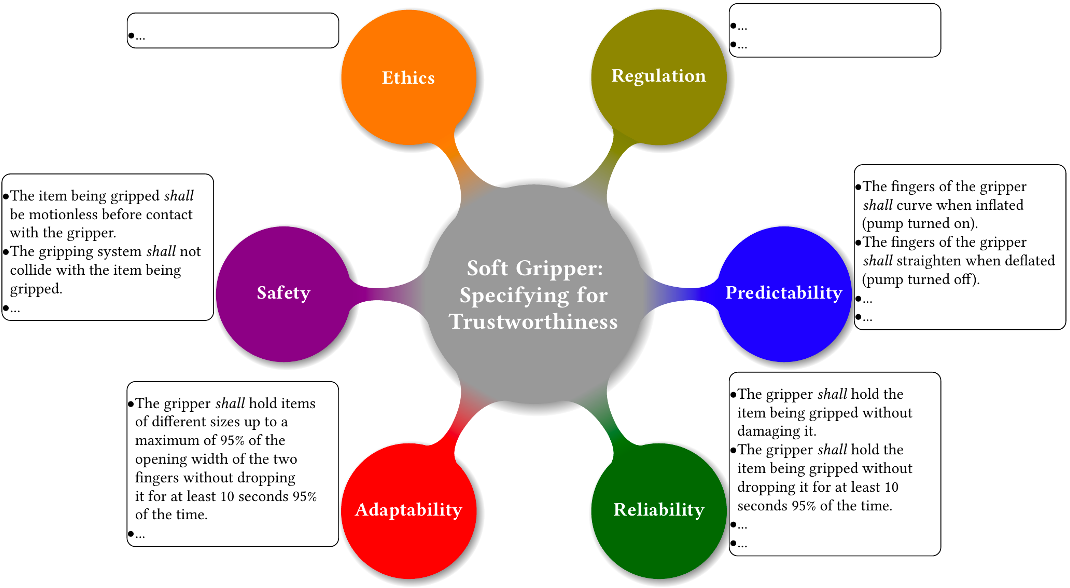
\includegraphics[width=0.9\textwidth]{figures/Fig1.png}
	\caption{Soft gripper: Specifying for trustworthiness (diagram to be provided...).}
	\label{SR-spec}
\end{figure*}

\subsection{Background}\label{background}
\subsubsection{Recycled Soft Gripper}

[Short Summary of recycled soft gripper paper by \cite{Partridge2022}, which is used in the current study]
\textbf{[Alix Partridge to provide this short subsection -- about 300 words]}
\\\\\\
\subsubsection{Pick-and-Place tasks of Grocery Items Case Study}
%Let us consider an automated warehouse, where items are picked from storage crates which then need to be placed in delivery crates for assembling and delivery. 
%The items vary in their shape, size, orientation and packaging which make the automation challenging. 
%Other challenges are constrained and relatively cluttered space to operate on; and fragile or deformable nature of certain items. 
%Furthermore, there can be the presence of other uncertainties, such as manufacturing inconsistencies; and temporal nature of the fabrics used in the gripper which can lead to degradation of performance. 
Let us consider an automated warehouse, where items are picked from storage crates which then need to be placed in delivery crates for assembling and delivery. 
There are several uncertainties that contribute to making the automation challenging: (i) items can vary in their shape, size, packaging, and orientation; (ii) fragile or deformable nature of certain items; (iii) constrained and relatively cluttered space to operate on; (iv) manufacturing inconsistencies; and (v) temporal nature of the fabrics used in the gripper which can lead to performance degradation. 

In the use case, we consider four \emph{classes} of items: (i) \emph{soft–fragile} items (e.g. cake, bread, strawberry, bayberry), (ii) \emph{soft–non-fragile} items (e.g. sponge), (iii) \emph{hard–fragile} items (e.g. light bulb, egg), (iv) \emph{hard–non-fragile} items (e.g. plastic spoon). 
The objects being picked can be regular-shaped (e.g. sphere, cube, cone, pyramid, cylinder) or irregular-shaped ones (e.g. strawberries).
%Soft finger can conform to the object’s surface with stable grasping and environmental endurance.
The robotic pick-and-place task can be structured into a pipeline of four main tasks: (i) pre-grasping, (ii) ascension (grasping), (iii) translation (transport), and (iv) descension (placement). 
An example is the grocery use case of Ocado, which is considered as the world's largest online only supermarket \cite{Triantafyllou2019, Sotiropoulos2018}. \\\\\\

\subsubsection{Standards}
Although no direct industry \textit{standards} have been defined for soft grippers so far, there are several standards in the area of rigid robotics that provide: (i) a set of terminology and definitions for robotic hands and grippers; and (ii) guidance into the safe spaces and distances gripping systems need to function. 

In 2018, a working group under the IEEE Technical Committee for Robotic Hands, Grasping and Manipulation proposed a standard \cite{Falco2018}, which provides a set of terminology and associated definition for robotic hands. % (see pg. 3 for a definition for soft robotics). 
%It covers terms relevant to defining performance for robotic hands. %\emph{Proposed Standard Terminology for Robotic Hands and Associated Performance Metrics} standard \cite{Falco2018} provides 
Meanwhile, \emph{ISO 14539:2000} standard  targets manipulating of industrial robots and provides terms to describe object handling and terms of functions, structures, and elements of grasp-type grippers \cite{ISO14539:2000}.
%focuses on the functionalities of end effectors and concentrates on grasp type grippers \cite{ISO14539:2000}. It specifically targets manipulating of industrial robots and provides terms to describe object handling and terms of functions, structures, and elements of grasp-type grippers.
\emph{ISO 10218-1} and \emph{ISO 10218-2} provide safety requirements for industrial robots and their integration. 
These standards provide safety guidance related to different spaces associated with a robot application (i.e. maximum, restricted, operating, safeguarded); speed and separation monitoring using detecting zones; and safety functions for end effector force and pressure. Similar guidance is provided in collaborative spaces of collaborative industrial robot systems in \emph{ISO/TS 15066}.
%Meanwhile, \emph{ISO/TS 15066} provides safety requirements for collaborative industrial robot systems and work environment (collaborative spaces). 

%speed and separation monitoring of 
%
%overview of different spaces associated with a robot application (i.e. maximum, restricted, operating, safeguarded)
%can provide some insights into the safe operation of soft grippers. 
%In this subsection, we highlight the main related standards to specifying a soft gripper. 




%These standards provides insights into the safe operation of a robotic gripper. ...
%In service robotics, \emph{ISO 13482 }covers the hazards presented by the robots and devices for applications in non-industrial environments for providing services. \emph{ISO 23482-1} and \emph{ISO 23482-2} standards extend ISO 13482 with guidance and methods that can be used to test personal care robots. ...

\subsection{Related Work}\label{relatedwork}
In \cite{Cheng2021}, the authors propose a three-finger soft-rigid gripper actuated by a soft pneumatic actuator for low-damage gripping of fragile and soft objects. 
By conducting a series of static and dynamic gripping tests that use different forces and fingertip displacements, the authors demonstrate the improved \textit{performance} and \textit{adaptability} of their gripper.  %linear-extension 

A new compliant soft robotic gripper is proposed in \cite{Liu2021} for grasping of objects and capping manipulations. This is through the coordination of its three soft fingers and in hand-manipulation. 
The core issue being addressed is \textit{adaptability} that achieves manipulative tolerance and dexterity for manipulating objects of various sizes, shapes,masses, and positions/orientations. 
The grasping tests conducted demonstrate that the soft finger can conform to the object’s surface with stable grasping and environmental endurance. 

In\cite{Chen2018}, the authors synthesize a soft cable-driven gripper by recasting its mechanical design as a topology optimization problem. 
They perform several fatigue, blocking force, and grasping tests to evaluate the \textit{performance} of their gripper.  
The results of the grasping tests reveal that their optimized gripper can handle a large range of unknown objects of different shapes and weights with different grasping modes (i.e. power grips, precision grips and a combination of both).

In another related work \cite{Cai2021}, a pneumatic webbed soft gripper has been developed and evaluated to grasp unstructured and fragile objects. 
The authors present the experimental results of grasping delicate objects (e.g. egg, strawberry, candy and knife) to demonstrate the \textit{safety} and \textit{adaptability} of their webbed soft gripper. % for fragile and crisp objects.

A reinforced soft gripper is proposed in \cite{Hwang2020} with a mechanically strengthened electro adhesion pad and a multi-layered dielectric elastomer actuator. The soft gripper has two fingers and can grasp various shapes of objects demonstrating its \textit{adaptability}, such as hexahedral, spherical, cylindrical, and flat structures. Also, it could hold up and move objects moving weighing 625 g by robotic manipulation. 

In \cite{Shin2021}, the authors propose a soft gripper for smart manufacturing that improves on the Fin Ray finger with improved gripping capability. The \textit{performance} as in gripping weight of the modified finger improved by 40\%. The authors perform gripping tests for a total of 17 types of objects, which could be rigid or soft.

As discussed, most existing works (e.g. \cite{Cheng2021,Liu2021,Chen2018,Cai2021,Hwang2020,Shin2021}) are largely on improving  \textit{adaptability} or \textit{performance} of a soft gripper. However, they do not cover a broad range of trustworthiness properties, as considered in our study. 
Furthermore, most existing approaches (e.g. \cite{Hong2022,Bhattacharya2019,Tadakuma2020,Loh2014,Nishikawa2019,Mohan2020}) only describe some parameters of the end-effector, and no work explores a wide-ranging specification for trustworthiness as proposed in our study.


%\subsubsection{Approaches on soft robotics specifications} 

%\subsubsection{Approaches on trustworthiness properties}[Draft]
%strawberry paper

% Modeling of a Soft-Rigid Gripper Actuated by a Linear-Extension Soft Pneumatic Actuator

%For achieving low-damage gripping to the object in static gripping system, we proposed a soft-rigidgripper actuated by a linear-extension soft pneumatic actuator in this study.
%
%Based on such studies, we proposed a soft-rigid gripper actuated by a linear-extension soft pneumatic actuator used in a static gripping system.
%
%In this study, we developed a three finger gripper with a built-in linear-extension soft pneumatic actuator and a slider link mechanism, as shown in Figure 1a.
%
%We proposed a soft-rigid gripper, which was actuated by a linear-extension softpneumatic actuator composed of a metal spring wound on the outer wall of a cylindricalsilicone cavity
%
%
%Furthermore,the low damage gripping to fragile and soft objects in static and dynamic gripping tests showed goodperformance of the gripper. Overall, the results indicated the potential application of the gripper inpick-and-place operations.
%
%Static gripping test:
%Before the gripping test, a pre-experimentwas conducted to test the minimum gripping force and fingertip displacement requiredfor the gripper to stably lift the above objects. The resulted values would be as the safethresholds of the gripping force and fingertip displacement.
%
%Figure 13. Static gripping test of the gripper for controlling gripping force and fingertip displacement. (a) Control thegripping force to 2 N to grip light bulb and raw egg, (b) control the fingertip displacement to 3 mm to grip bread and cake,and (c) control the gripping force to 1 N or the fingertip displacement to 1 mm to grip strawberry and bayberry.
%
%
%Dynamic gripping test:
%In addition to proving the static gripping performance of the gripper in Section 5.4,we conducted an experiment to further demonstrate that the gripper has certain dynamicgripping ability for vulnerable objects in Figure 14.
%
%
%Dynamic gripping test of the gripper. (a) The movement path of the gripper in the dynamic gripping test wasdivided into ascension, translation, and descension, (b) the gripper had two movement states at each movement path,(c) The image snapshots of the dynamic gripping of the gripper under different times at the acceleration of 150 mm/s2.

%-----------------------------------------------------------------------------------------------------------------------------------------

%
%
%%In \cite{Liu2021}, the authors present a new compliant soft robotic gripper for objects handling and cap manipulation through the coordination of three soft fingers and in-hand manipulation.... 
%%Soft Robotic Gripper Driven by Flexible Shafts for Simultaneous Grasping and In-Hand Cap Manipulation
%This study presents a new compliant soft robotic gripper for objects handling and cap manipulation through the coordination of three soft fingers and in-hand manipulation. 
%The experiments are conducted to validate that the soft robotic gripper can successfully realize simultaneous grasping and capping manipulations with only one flexible shaft actuation for every single soft finger.
%ROBOTIC grippers interacting with unstructured tasks experience a core issue, that is, adaptability [1]. A robotic gripper with adaptability realizes manipulative tolerance and dexterity for manipulating objects with various sizes, shapes,masses, and positions/orientations.
%Main contributions: 
%1) A robotic gripper consists of soft fingers that achieve in-hand simultaneous exertion of bending and tangential force/torque and can exhibit environment tolerance, such as impact and puncture.
%2) A soft finger is controlled by a single flexible shaft to achieve bending and twisting DoFs, which are essential for the simultaneous exertion of grasping and in-hand capping manipulation.
%--
%Fig. 9 shows the utility of the soft robotic gripper ingrasping different objects. The objects involved have variousshapes, masses, and sizes, and are used every day, as shownin Fig. 9(b)–(h). An irregular object being grabbed at the palmof the robotic gripper is released later on by the soft fingers.Each task was conducted five times, and all grasps wereaccomplished. Fig. 9(i)–(k) shows the different directionaldisturbance forces on the objects (cup, bottled water, andglossy glass bottle) that are power-grasped (see an experimentalvideo in the supplementary materials). The experimentsdemonstrated that the soft robotic gripper could successfullygrasp different objects with various shapes, masses, and sizes.The soft finger can conform to the object’s surface with stablegrasping and environmental endurance. The specification ofthe grasps on objects is presented in Table II.The performance of the loosening capped object is evaluatedto verify the twisting capability of the soft robotic gripper.The robotic gripper performs uncapping manipulation on acapped cup through the cooperation of the three soft fingers.

%-----------------------------------------------------------------------------------------------------------------------------------------
%Topology Optimized Design, Fabrication, and Characterization of a Soft Cable-Driven Gripper
%In this work, the authors synthesize a soft cable-driven gripper by recasting its mechanical design as a topology optimization problem.
%The experimental tests show that the optimized gripper can handle a large range of unknown objects with different grasping modes (power grips, precision grips or combination of them).
%
%The experiments show thatthe gripper can handle a large range of unknown objects of differentshapes and weights (up to 1 kg), with different grasping modes.
%
%In this letter, we develop a soft cable-driven gripper using thelevel set-based topology optimization method. 
%
%
%size, weight, shape regularity, hardness...
%
%It isobserved that the gripper may present different grasping mode,i.e., power grips, precision grips or combination of them.
%
%We have applied the level set-based optimization approach tosynthesize a soft gripper. By modelling the interactions betweenthe gripper and objects as the boundary conditions and appliedloads, the mechanical design problem is recast as a mathematicaloptimization problem. The experimental tests show that theoptimized gripper can handle a large range of unknown objectswith different grasping modes.
%-----------------------------------------------------------------------------------------------------------------------------------------
%Pneumatic Webbed Soft Gripper for Unstructured Grasping
%In this study, a pneumatic webbed soft gripper to grasp unstructured and fragile objects was developed and evaluated. 
%Inspired by duck foot and octopus tentacle, a pneumatic webbed soft gripper was proposed, which is consisted of four multi-chambered fingers and four webs. 
%Figure shows the experimental results of grasping delicate objects of egg, strawberry, candy and knife. 
%The successful grasping of egg and strawberry demonstrated the safety and adaptability of the webbed soft gripper for fragile and crisp objects, especially food and agricultural products.
%
%
%This work tried to develop a soft gripper that can hold multiplediminutive objects in one snatch and improve the stability andreliability of grasping. The study proposed a four-finger webbedsoft gripper and focused on the design, fabrication, and control.The design inspiration came from the structure of the flippers ofducks, i.e., adding webs to the traditional soft fingers to wrap theobjects when grasping them. The webbed soft gripper caneffectively prevent the gripped objects from falling off from thegaps between the fingers, and reduce the precision requirements ofthe capture operation, which greatly improves the success rate andreliability of grasping.
%
%
%Figure 15 shows the experimental results of grasping delicateobjects of egg, strawberry, candy and knife. The successfulgrasping of egg and strawberry demonstrated the safety andadaptability of the webbed soft gripper for fragile and crisp objects,especially food and agricultural products. For the candy graspingexperiment, 50 times grasping were executed for a pile of candiesin a basket, as shown in Figure 15c. On average, there were 4candies grabbed for each try, which can hardly be realized withoutthe web. The packing effects of the web were also demonstratedby grasping the versatile knife without precise orientation orposition, as shown in Figure 15d.
%


%-----------------------------------------------------------------------------------------------------------------------------------------
%Mechanically Strengthened Electroadhesion based Soft Gripper with Multi-layered Dielectric Elastomer Actuator
%In \cite{Hwang2020}, the authors introduce a reinforced soft gripper with a mechanically strengthened electro adhesion pad and a multi-layered dielectric elastomer actuator, for a practical robotic application... In 

%With this study, we demonstrate dynamic pickingand placing tasks with the proposed gripper assembled in arobotic system.
%
%
%In this paper, we propose a reinforced soft grippercomposed of a mechanically strengthened electroadhesionpad and a multi-layered DE bending actuator. Theelectroadhesion pad is comprised of a metallic electrodepattern printed on thin polyimide film. This polyimide film isflexible but has a very high elastic modulus compared withtypical soft materials for a DE gripper, such aspolydimethylsiloxane (PDMS) and acrylic elastomer.Moreover, to increase the bending force which is used forgrasping, a multi-layered DE actuator has been applied to aunimorph structure. In addition, a uniform deformation of theproposed gripper is induced by an aligned metallic electrodepattern and expansion of the DE actuator layers.For maximizing the performance of the proposed grippersystem, we optimized the electrode pattern in aspects of thethickness of the insulation layer. In addition, we analyzed thenumber of layers of the multi-layered DE actuator. Finally,the proposed soft gripper practically picks up and placesobjects of various shapes weighing up to 625 g, for a realrobotic application.
%
%
%The soft gripper is composed of two soft fingers, whichare designed based on the process above. This soft grippercan hold up various shapes of target objects, includinghexahedral, spherical, cylindrical, and flat structures
%
%These results confirm that the designed softgripper can be widely used to pick and place random objectsthanks to its adaptability, stability and high capability.

%-----------------------------------------------------------------------------------------------------------------------------------------
%A Universal Soft Gripper with the Optimized Fin Ray Finger


%Furthermore, formulating specifications of soft robotic grippers has received very little attention by the soft robotics community where most existing works only describe some parameters of the end-effector (e.g. \cite{Hong2022,Bhattacharya2019,Tadakuma2020,Loh2014,Nishikawa2019,Mohan2020}). 
%


%Also, these works do not provide a wide-ranging specification for trustworthiness as our work...\\.
%Existing works proposed on soft robotics grippers provide specifications of some dimensions of parameters of an end-effector, such as size, height, weight, width, depth, material dimensions \cite{Hong2022,Bhattacharya2019,Tadakuma2020,Loh2014,Nishikawa2019,Mohan2020}. ...



%Approaches on pick-and-place tasks (e.g. SoMa project and Ocado grocery example) \cite{Negrello2020,Triantafyllou2019,Sotiropoulos2018, Pozzi2016,Bianchi2018}...

\section{Specification of a Soft Gripper}\label{specification-gripper}
%Trustworthiness of a soft gripper can be dependent on both functional and non-functional properties, such as predictability, reliability, adaptability and safety. 
%These properties are especially significant for a soft gripper in situations such as ...

In our study, we consider several functional and non-functional properties for trustworthiness of a soft gripper, such as predictability, reliability, adaptability, safety, ethics and regulation.
%However, with respect to safety of a soft gripper, we consider safety from the viewpoint of the item being gripped...
%...


\subsection{Predictability}\label{predictability}
\emph{Predictability} concerns the ability of a system or component to perform its tasks as expected (stereotypical) without any surprises to a human. % reliably. ...
\begin{itemize}
	\item RQ1.1: The fingers of the gripper \emph{shall} curve when inflated (pump turned on).  
	\item RQ1.2: The fingers of the gripper \emph{shall} straighten when deflated (pump turned off).  
	\item RQ1.3: The curvature of a finger \emph{shall} be proportional to its internal pressure. 
	\item RQ1.4: The fingers \emph{shall} be in a stable state -- pre-pressurized/inflated 10 times, prior to being used.  
	\item RQ1.5: The fingers \emph{shall} be inflated with a pressure between 3-4 psi pressure range. \emph{(Note: \cite{Partridge2022})}
	\item RQ1.6: The fingers \emph{shall} be inflated with a flow rate between 2-3.2 L/min range. \emph{(Note: \cite{DEWIN2022})} 
\end{itemize}

%\begin{center}
%	\begin{tabular}{|p{7mm}|p{72mm}|}
%		\hline
%		RQ1.1 & The fingers of the gripper \emph{shall} curve when inflated (pump turned on).  \\ 
%		\hline
%		RQ1.2 & The fingers of the gripper \emph{shall} straighten when deflated (pump turned off).  \\ 
%		\hline
%		RQ1.3 & The curvature of a finger \emph{shall} be proportional to its internal pressure. \\
%		\hline
%		RQ1.4 & The fingers \emph{shall} be in a stable state -- pre-pressurized/inflated 10 times, prior to being used. \\ 
%		\hline
%		RQ1.5 & The fingers \emph{shall} be inflated with a pressure between 3-4 psi pressure range. \emph{(Note: \cite{Partridge2022})} \\
%		\hline
%		RQ1.6 & The fingers \emph{shall} be inflated with a flow rate between 2-3.2 L/min range. \emph{(Note: \cite{DEWIN2022})} \\	[1ex] 		
%		\hline
%	\end{tabular}
%\end{center}

\subsection{Reliability}\label{reliability}
\emph{Reliability} is defined as the ``ability of a system or component to perform its required functions under stated conditions for a specified period of time" \cite{ISO24765:2017}. 
%\begin{center}
%	\begin{tabular}{|p{7mm}|p{72mm}|}
%		\hline
%		RQ2.1 & The gripper \emph{shall} hold the item being gripped without damaging it.  \\ 
%		\hline
%		RQ2.2 & The gripper \emph{shall} hold the item being gripped without dropping it for at least 10 seconds 95\% of the time.  \emph{(Note: \cite{Sotiropoulos2018}, pg. 652))}\\ 
%		\hline
%		RQ2.3 & The gripper \emph{shall} successfully maintain grasp during translation of the gripped item for a maximum velocity and acceleration of 0.03 m/s and 150 mm/s$^2$. \emph{(Note: \cite{Triantafyllou2019}, pg. 5; \cite{Cheng2021}, pg. 15))}\\
%		\hline
%		RQ2.4& The gripper \emph{shall} successfully grasp when the rate of inflation is in the range of 2-3.2 L/min. \emph{(Note: \cite{DEWIN2022})}\\
%		\hline
%		RQ2.5 & [\emph{Graceful degradation}] The gripper \emph{shall} experience $\le$ 5\% increase in dropping of an item across 100 hours of operation. (comment by SW: consider degradation rate instead?) \\			\hline	
%		RQ2.6 & [\emph{Graceful degradation}] The gripper \emph{shall} experience $\le$ 5\% increase in damaging of an item across 100 hours of operation.  (comment by SW: consider degradation rate instead?) \\		[1ex] 		
%		\hline
%	\end{tabular}
%\end{center}
\begin{itemize}
	\item RQ2.1: The gripper \emph{shall} hold the item being gripped without damaging it. 
	\item RQ2.2: The gripper \emph{shall} hold the item being gripped without dropping it for at least 10 seconds 95\% of the time.  \emph{(Note: \cite{Sotiropoulos2018}, pg. 652))}
	\item RQ2.3: The gripper \emph{shall} successfully maintain grasp during translation of the gripped item for a maximum velocity and acceleration of 0.03 m/s and 150 mm/s$^2$. \emph{(Note: \cite{Triantafyllou2019}, pg. 5; \cite{Cheng2021}, pg. 15))}
	\item RQ2.4: The gripper \emph{shall} successfully grasp when the rate of inflation is in the range of 2-3.2 L/min. \emph{(Note: \cite{DEWIN2022})}
	\item RQ2.5: [\emph{Graceful degradation}] The gripper \emph{shall} experience $\le$ 5\% increase in dropping of an item across 100 hours of operation. (comment by SW: consider degradation rate instead?) 
	\item RQ2.6: [\emph{Graceful degradation}] The gripper \emph{shall} experience $\le$ 5\% increase in damaging of an item across 100 hours of operation.  (comment by SW: consider degradation rate instead?) 
\end{itemize}


\subsection{Adaptability} \label{adaptability}
\emph{Adaptability} is defined as the ``degree to which a product or system can effectively and efficiently be adapted for different or evolving hardware, software or other operational or usage environments" \cite{ISO24765:2017}. 
\begin{itemize}
	\item RQ3.1: The gripper \emph{shall} hold items of different sizes up to a maximum of 95\% of the opening width of the two fingers without dropping it for at least 10 seconds 95\% of the time.
	\item RQ3.2: The gripper \emph{shall} hold items of different shapes (e.g. sphere, cube, cone, pyramid, cylinder) without dropping it for at least 10 seconds 95\% of the time.
	\item RQ3.3: The gripper \emph{shall} hold items, which can be of regular or irregular shape, without dropping it for at least 10 seconds 95\% of the time. 
\end{itemize}
%\begin{center}
%	\begin{tabular}{|p{7mm}|p{72mm}|}
%		\hline
%RQ3.1 & The gripper \emph{shall} hold items of different sizes up to a maximum of 95\% of the opening width of the two fingers without dropping it for at least 10 seconds 95\% of the time. \\
%\hline
%RQ3.2 & The gripper \emph{shall} hold items of different shapes (e.g. sphere, cube, cone, pyramid, cylinder) without dropping it for at least 10 seconds 95\% of the time. \\[1ex] 
%\hline
%RQ3.3 & The gripper \emph{shall} hold items, which can be of regular or irregular shape, without dropping it for at least 10 seconds 95\% of the time. \\ 
%\hline
%
%
%RQ3.4 & The gripper \emph{shall} hold an item independent of its orientation without dropping it for at least 10 seconds 95\% of the time. \\ 	 
%\hline
%\emph{\sout{RQ3.5}} & \emph{\sout{Non-symmetrical objects \emph{shall} be successfully grasped (no slipping) when it is picked with X–Y* rotational offset for at least 10 seconds 95\% of the time.}}  \\ 
%\hline
%\emph{\sout{RQ3.6}} & \emph{\sout{Non-symmetrical objects \emph{shall} not be dropped when it is picked with X–Y* rotational offset for at least 10 seconds 95\% of the time.}}\\
%\hline
%\emph{\sout{RQ3.7}} & \emph{\sout{Non-symmetrical objects \emph{shall} not be damaged when it is picked with X–Y* rotational offset for at least 10 seconds 95\% of the time.}}\\
%\hline
%\emph{\sout{RQ3.8}} & \emph{\sout{For non-symmetrical objects, the grasping contact position (focus) of the gripper \emph{shall} be $\le$ X mm from the centre of the mass of the object. (Note: gripper pose agnostic, does not need to be captured).}}\\	[1ex] 
%\hline
%	\end{tabular}
%\end{center}


\subsection{Safety}\label{safety}
\emph{Safety} is defined as an ``expectation that a system does not, under defined conditions, lead to a state in which human life, health,property, or the environment is endangered" \cite{ISO24765:2017}. 
In our study, we consider safety from the perspective of the item being gripped and not from the physical harm to a human.
\begin{itemize}
	\item RQ4.1: The item being gripped \emph{shall} be motionless before contact with the gripper. 
	\item RQ4.2: The gripping system \emph{shall} not collide with the item being gripped. 
	\item RQ4.3: The gripping system \emph{shall} only make contact with the item using the gripper.
	\item RQ4.4: When grasping a hard–fragile item (e.g. light bulb, raw egg), the soft actuator \emph{shall} be inflated until the gripping force does not exceed 2N. \emph{(note: \cite{Cheng2021}, pg. 14)}
	\item RQ4.5: When grasping a soft–fragile item like cake or bread, the soft actuator \emph{shall} be inflated until the fingertip displacement does not exceed 3mm. \emph{(note: \cite{Cheng2021}, pg. 14)}
	\item RQ4.6: When grasping a soft–fragile item like strawberry or bayberry, the soft actuator \emph{shall} be inflated until the gripping force does not exceed 1N and the fingertip displacement does not exceed 1mm. \emph{(note: \cite{Cheng2021}, pg. 14)}
\end{itemize}
%\begin{center}
%	\begin{tabular}{|p{7mm}|p{72mm}|}
%		\hline
%		RQ4.1 & The item being gripped \emph{shall} be motionless before contact with the gripper.   \\ 
%		\hline
%		RQ4.2 & The gripping system \emph{shall} not collide with the item being gripped. \\ 
%		\hline
%		RQ4.3 & The gripping system \emph{shall} only make contact with the item using the gripper.\\
%		\hline
%		RQ4.4 & When grasping a hard–fragile item (e.g. light bulb, raw egg), the soft actuator \emph{shall} be inflated until the gripping force does not exceed 2N. \emph{(note: \cite{Cheng2021}, pg. 14)}\\
%		\hline
%		RQ4.5 & When grasping a soft–fragile item like cake or bread, the soft actuator \emph{shall} be inflated until the fingertip displacement does not exceed 3mm. \emph{(note: \cite{Cheng2021}, pg. 14)}\\
%		\hline
%		RQ4.6 & When grasping a soft–fragile item like strawberry or bayberry, the soft actuator \emph{shall} be inflated until the gripping force does not exceed 1N and the fingertip displacement does not exceed 1mm. \emph{(note: \cite{Cheng2021}, pg. 14)}\\	[1ex] 
%		\hline
%	\end{tabular}
%\end{center}

\subsection{Ethics}\label{ethics}
[\textbf{Arianna Manzini. Maximum: 675 words.}]

\subsection{Regulation}\label{regulation}
[\textbf{Peter Winter. Maximum: 675 words.}]

\section{Discussion and Conclusions} \label{discussion-conclusions}



...
\paragraph{Verifiability} 
[Draft]
In this subsection, we will discuss how we propose to make the requirements verifiable (raw requirements to verifiable requirements, and explain the delta)...

System engineers need to design the system for \textit{verifiability}, as the ultimate purpose of specifications is verifying that the end product exhibits the intended properties \cite{Gerson1993}. This requires the intended properties to be demonstrable, i.e. that knowledge of the end result needs to be attainable. Avoiding negative requirements and including numerical tolerances are not the only means of writing requirements for verifiability.  ...

The notion of \emph{verifiability} is considered key for improving trustworthiness of an AS (e.g. soft robot) \cite{Mousavi2022}. 
A unified and holistic approach to verifiability will fundamentally change the approach to verification of ASs and it will lead to systems that are by their construction are worthy of our trust. 
The key insight here is that verifiability can be achieved by considering verification early, for example during specification and system design. 
To this end, one can seek to promote verifiability to a first-class system design objective \cite{Eder2021}. ...

For a system to be {\em verifiable\/}, a person or a tool needs to be able to check its correctness~\cite{ISO24765:2017} with respect to its requirements and specification \cite{Abeywickrama2022}. 
The main challenge is in specifying and designing the system in such a way that this process is made as easy and intuitive as possible.
%
For ASs in particular, specific challenges include 
%
(i) capturing and formalizing requirements including functionality, safety, security, performance and, beyond these, any additional non-functional requirements purely needed to demonstrate trustworthiness; 
%	 
(ii) handling flexibility, adaptation and learning; and 
%
(iii) managing the inherent complexity and heterogeneity of both the AS and the environment it operates in. 

Specifications need to represent the different aspects of the overall system in a way that is natural to domain experts, facilitates modelling and analysis, provides transparency of how the AS works and gives insights into the reasons that motivate its decisions. 
%
To specify for verifiability, a specification framework will need to offer a variety of domain abstractions to represent the diverse, flexible and possibly evolving requirements ASs are expected to satisfy. 
%
Furthermore, the underlying verification framework should connect all these domain abstractions to allow an analysis of their interaction. This is a key challenge in specification for verifiability in ASs.

\begin{itemize}
	\item Describe above in the context of a soft gripper – how we can consider above i––iii when specifying for trustworthiness for a soft gripper.
	\item Also, how we can provide for domain abstractions...
\end{itemize}
...\\


%Discuss how the requirements in the specification can be made verifiable. Discuss raw requirements... verifiable version and the delta...
%Usability and Verifiability of Secure Features for Authenticating Identity
%Verifiability differs from verification that in verifiability it is unknown at the start what is the level of verification can be done to the feature.
%
%
%Verifiability differs from verification that in verifiability it is unknown at the start
%what is the level of verification can be done to the feature.
%
%Verification should be raised to a design concern, which is what verifiability is about. 
%So do not state requirements that you don't know how to verify the moment state to requirement. You need to confirm how you would verify it.
%And if you can't do that, it's not worth it.
%
%the generic version, and then the instantiation...
%
%How do you make this verifiable? Well, in order to make it verifiable, we need to know these things, and here is a refined version of this step we can deem verifiable because we've now instantiated it. But look at 1.5 and 1.5 in the original requirements.
%
%Raw version.. verifiable version...
%delta for 
%
%what a proper  curve shall be or what is straightness
%
%to make a verifiable spec what needs to do
%
%visible the delta... raw sets of reqts.. purpose of this section.. skim them how would i do it... KE
%what are the techniques 
%process should go through
%
%change between the original raw instantiation of raw specification
%designer, req eng... question is how do you verify it
%designer might come up with an idea
%
%what the delta is between the raw and the what we consider verifiable
%
%purpose of this section is to highlight that that's not enough to to make verifiability


\cite{Cheng2021,Bhattacharya2019,Bianchi2018,Cai2021,Chen2018,Hong2022,Farrell2022,Hwang2020,Liu2021,Loh2014,Mohan2020,Negrello2020,Nishikawa2019,Pozzi2016,Shin2021,Sotiropoulos2018,Tadakuma2020,Triantafyllou2019}


\section*{Acknowledgments}
The work presented in this paper has been supported by the UK Engineering and Physical Sciences Research Council (EPSRC) under the grant [EP/V026518/1].

\bibliographystyle{IEEEtran}
\bibliography{Spec-SoftRobotics-Bibliography.bib}

\newpage

\vfill

\end{document}